\documentclass[8pt,t]{beamer}


\usepackage[PunctStyle=banjiao]{xeCJK}
\setCJKsansfont{Noto Sans CJK SC}
\setCJKmainfont{Noto Serif CJK SC}
\setCJKmathfont{Noto Serif CJK SC}
\setlength{\parindent}{2em}
\usepackage{amsmath}
\usepackage{graphicx}
\usepackage{xcolor}
\usepackage{ulem}
\usepackage{CJKfntef}
\newcommand{\passthrough}[1]{#1}
\usepackage{hyperref}
\hypersetup{
	colorlinks=true,
	linkcolor=cyan,
	filecolor=cyan,
	urlcolor=cyan,
	citecolor=cyan,
}

% metadata
\date{\today}
\title{GNU/Linux for daily use}
\subtitle{ {它很好玩,我也要玩} {自由,开放,包容,协作.} }
\author{spinach/hehelego}
\institute{GeekPie@ShanghaiTech}

% beamer settings
\usetheme{Madrid}
\usecolortheme{seahorse}
\RequirePackage{geometry}
\setbeamersize{text margin left=.3cm}
\setbeamersize{text margin right=.3cm}
\setbeamerfont{footnote}{size=\tiny}

\begin{document}


\begin{frame}
	\titlepage{}
\end{frame}

\begin{frame}
	\frametitle{Sample}

	In this slide, some important text will be\footnote{footnote will be here}
	\alert{highlighted} because it's important.
	Please, don't abuse it.

	\begin{block}{Remark}
		Sample text
	\end{block}

	\begin{alertblock}{Important theorem}
		Sample text in red box
	\end{alertblock}

	\begin{examples}
		Sample text in green box. The title of the block is ``Examples''.
	\end{examples}
\end{frame}

\begin{frame}
	\frametitle{这是什么\quad About\footnote{Provided under the \textbf{CC0 Lincense}, and \href{https://github.com/hehelego/GnuLinux_for_daily_use}{\color{blue}{available on github}}}}

	\textcolor{gray}{\tiny{\sout{Linux日常使用、开发环境、服务维护的相关教程、书籍、博客等资料,随便一搜就是一大把.不要给geekpie workshop灌水啊}}}\\
	我不打算做复读机,只是尝试说服你:使用它是有必要的,使用它是可行的.\\
	当然这次分享不可避免地,会有一些GNU/Linux相关的基础介绍和使用技巧.

	\vspace{15em}
	\pause

	有些东西并不是那么难,只是你需要一个契机.\\
	让你意识到: 它很好玩,开始玩它并没有什么门槛.\\
	给你想要开始玩它的冲动. 这就是我要做的.\\

\end{frame}

\begin{frame}
	\frametitle{TOC}
	\begin{block}{这次分享中\uline{不会有}的东西}
		\begin{itemize}
			\item 如何安装一个GNU/Linux发行版,完成基础的配置
			\item 如何自己定制,编译并安装linux kernel
			\item 详细的GNU/Linux开发,运维指南
			\item android,embedded OS,domain-specific OS
			\item 如何在GNU/Linux环境下进行iOS开发,进行win32开发
			\item 传教/圣战 \sout{你们啊 不要总想着搞个大新闻 把我批判一番}
		\end{itemize}
	\end{block}

	\begin{block}{这次分享中\uline{包含}的内容}
		\begin{itemize}
			\item 对GNU/Linux的架构,社区,软件生态的简要介绍
			\item 为什么GNU/Linux可以满足你的日常使用需求
			\item \sout{虽然不完全正确但并非错得离谱的}入坑指南
		\end{itemize}
	\end{block}

	\pause
	\centering{
		\sout{The outline is omitted}\\
		``反复翻看目录的,不是真正的读者.''
	}
\end{frame}


\begin{frame}[c]
	\centering
	So, Let's get started
\end{frame}

%%%%%%%%%%%%%%%%%%%%%%%%%%%%%%%%%%%%%%%%%%%%%%%%%%%%%%%%%%%%%%%%%%%%%%%%%%%%%%%%%%%%%%%%%%%%%%%%%%
%%%%%%%%%%%%%%%%%%%%%%%%%%%%%%%%%%%%%%%%%%%%%%%%%%%%%%%%%%%%%%%%%%%%%%%%%%%%%%%%%%%%%%%%%%%%%%%%%%

\begin{frame}
	\frametitle{GNU/Linux,\ a brief introduction}
	目前,只有GNU/Linux和相关的外围生态,可以提供可以提供同时满足eoffice\&content creator\&developer\&system admin需要的环境.\\
	\pause 正如你所想的那样,这是我钦定的

	\pause
	\begin{block}{\sout{背书和念稿,这个我也会}}
		\begin{itemize}
			\item \sout{早都知道了的} 历史趣闻故事
			\item \sout{不会quiz到的} 操作系统层次
		\end{itemize}
	\end{block}

	\pause
	
\includegraphics[width=0.4\textwidth]{gnulinux-logo.png}
	
\includegraphics[width=0.4\textwidth]{foss.jpg}\\
	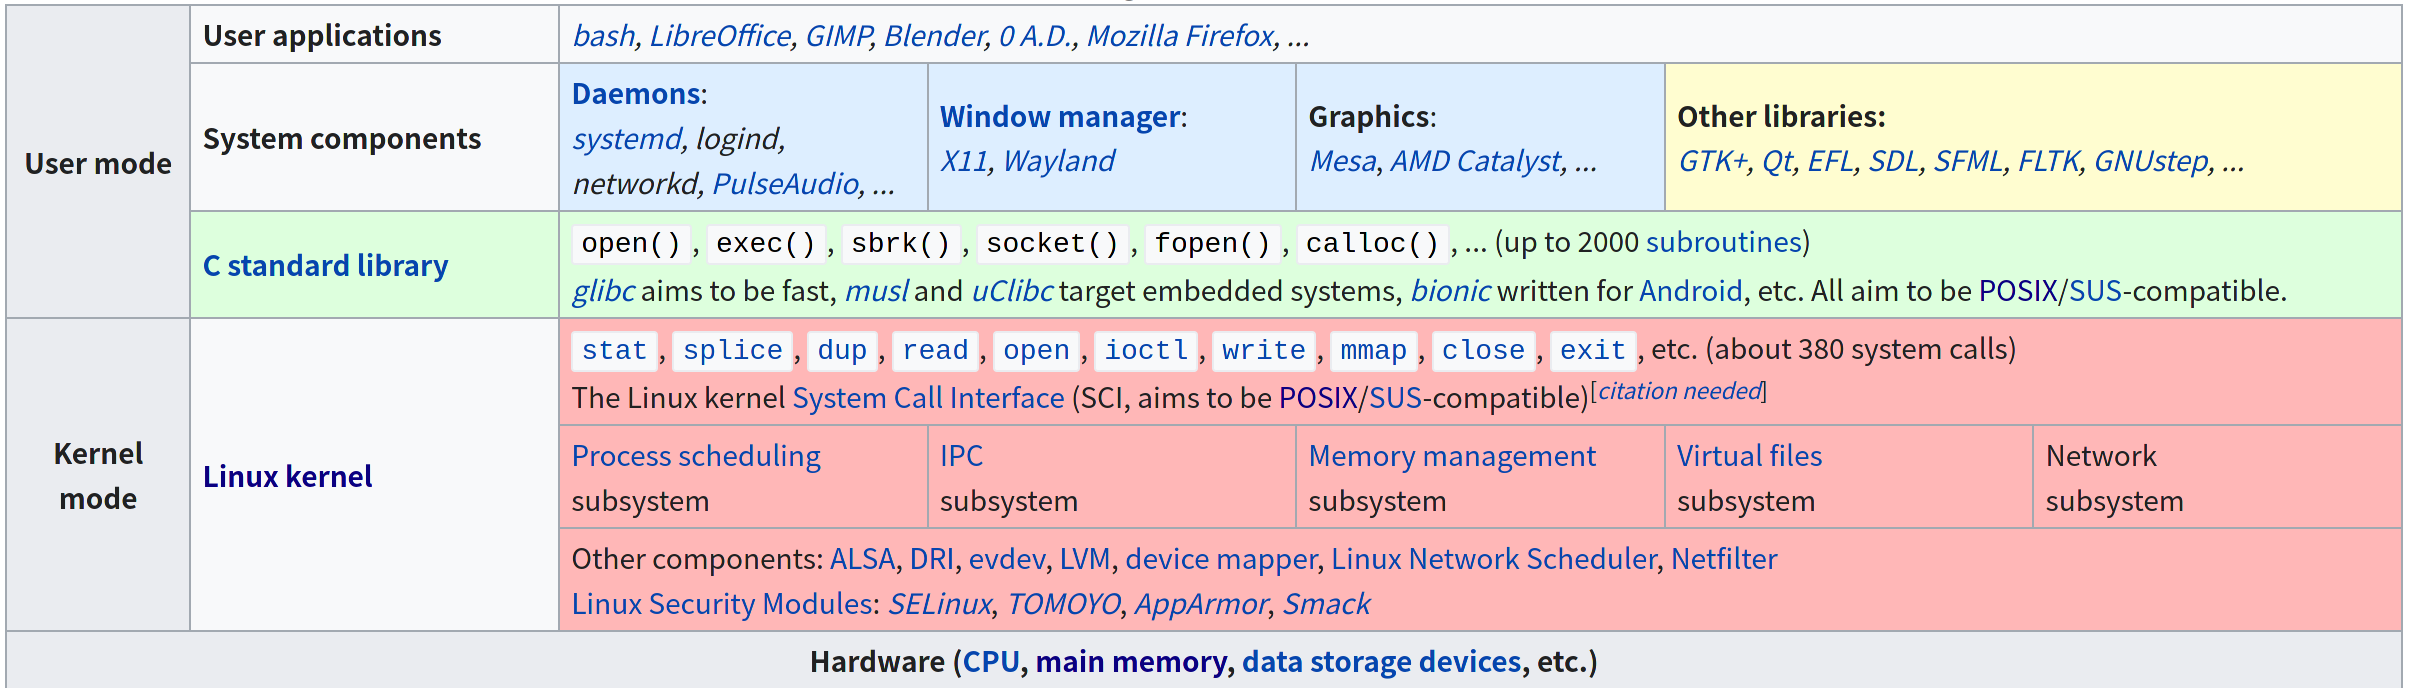
\includegraphics[width=0.4\textwidth]{linux-system.png}
	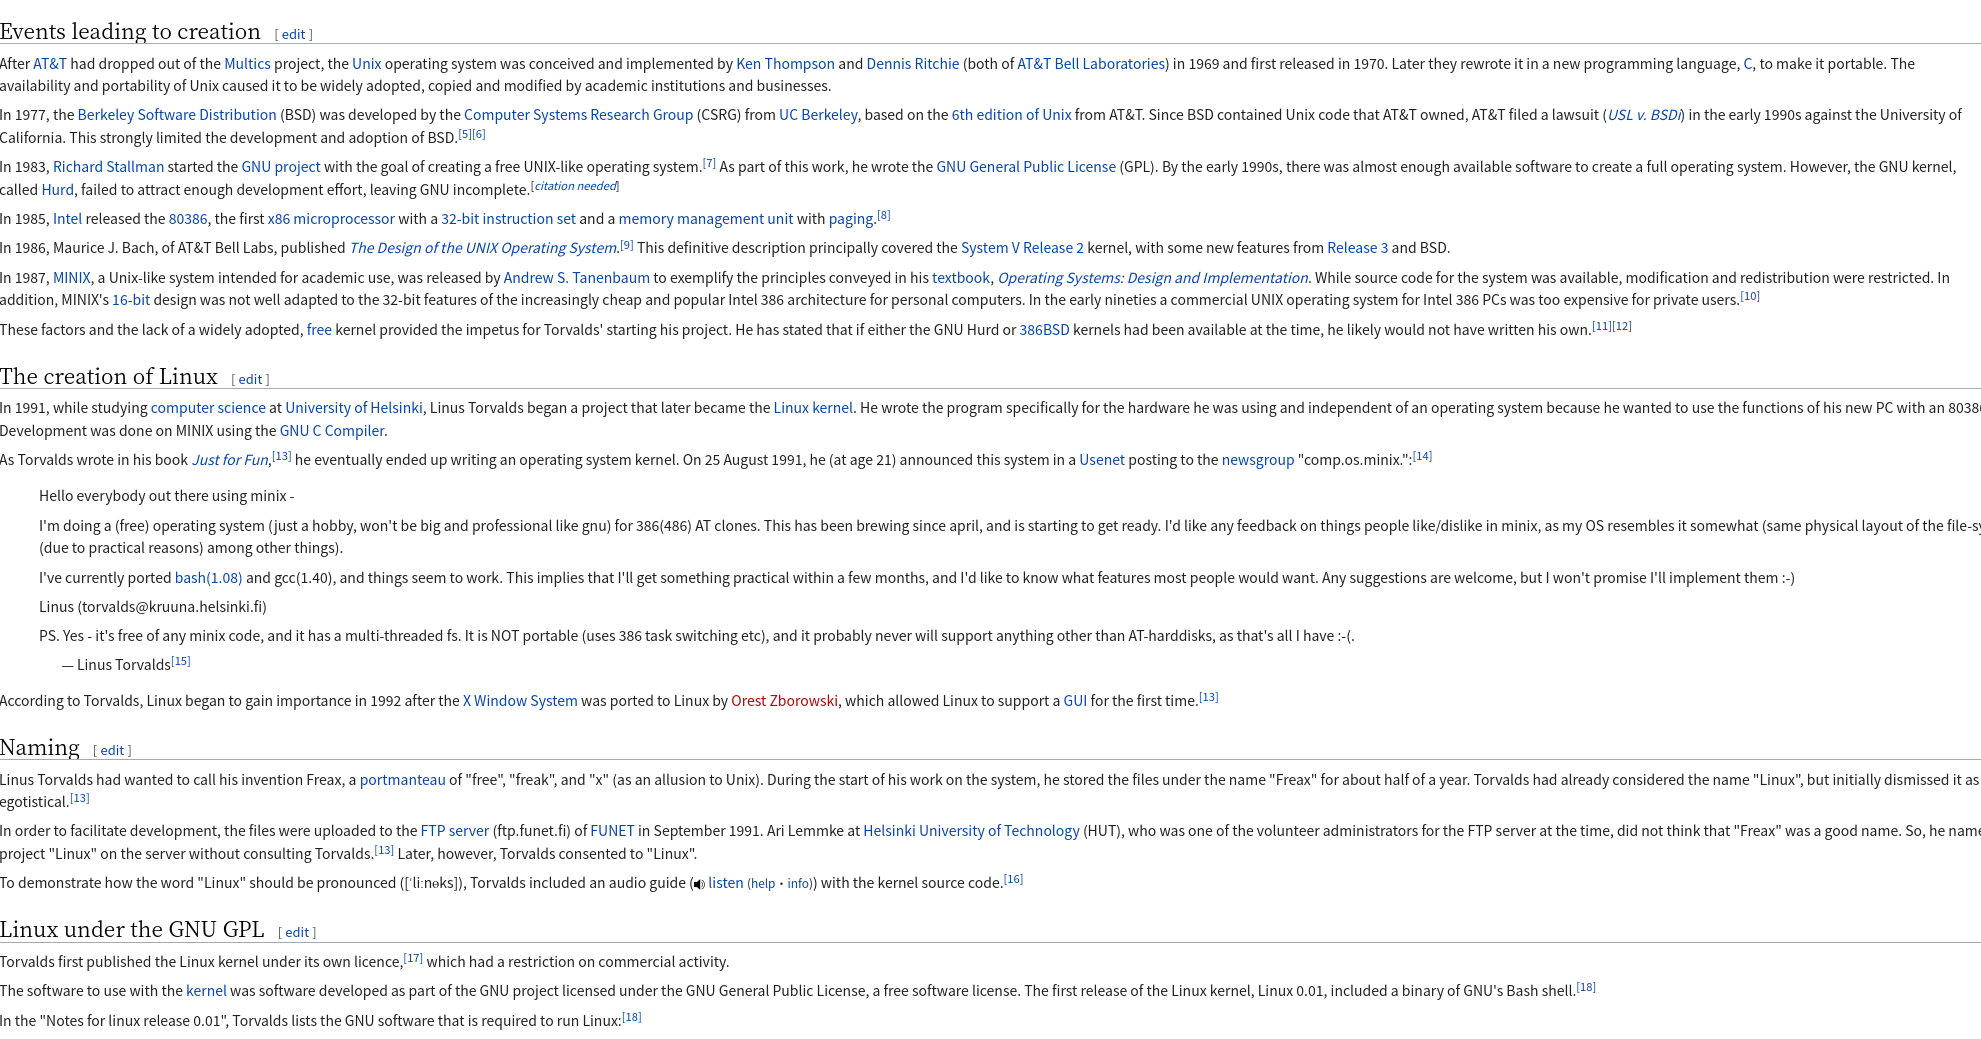
\includegraphics[width=0.4\textwidth]{history.png}

\end{frame}

%%%%%%%%%%%%%%%%%%%%%%%%%%%%%%%%%%%%%%%%%%%%%%%%%%%%%%%%%%%%%%%%%%%%%%%%%%%%%%%%%%%%%%%%%%%%%%%%%%
%%%%%%%%%%%%%%%%%%%%%%%%%%%%%%%%%%%%%%%%%%%%%%%%%%%%%%%%%%%%%%%%%%%%%%%%%%%%%%%%%%%%%%%%%%%%%%%%%%

\begin{frame}
	\frametitle{GNU/Linux, for daily use}

	\sout{我们钦定GNU/Linux是适合日常办公学习;}\\
	\sout{并且,可以在其上轻松搭建开发者,内容创作者,系统维护者所需的环境.}\\
	\sout{所以使用它是理所应当.}

	\pause

	\begin{block}{为何? 使用GNU/Linux}
		\begin{itemize}
			\item 100 percent controllable
			\item 100 percent customizable
			\item embrace FOSS,community driven,decentralized
			\item for fun, for working efficiently, or for anything.
		\end{itemize}
		最关键的是,你将拥有选择的权利.\\
	\end{block}

	\pause

	\begin{alertblock}{听说有锅啊}
		\begin{itemize}
			\item 安装光盘去哪里买啊;光驱怎么搞啊?
			\item 装啥都make,make install,自己编译自己管理依赖,麻烦死了;没源码装不了啊?
			\item 硬件兼容性不好,适配不好,屏幕撕裂,分辨率不可调?
			\item 动不动就kernel panic,稳定使用怎么可能?
			\item 出锅都要自己hack,而且完全没有中文资料,劝退
			\item \dots
		\end{itemize}
	\end{alertblock}
\end{frame}

\begin{frame}
	\frametitle{GNU/Linux, for daily use\quad (Cont'd)}

	\begin{block}{大人,时代变了!}
		naive 不要听风就是雨.
		\begin{itemize}
			\item 无脑安装,开箱即用, 有手就行.
			\item 系统维护,硬件驱动,GUI;安装,配置,使用? 认准apt/dnf/pacman.
			\item LTS,rc,hacked kernel随便选,甚至还能稳定+新特性全都要.
			\item arch wiki, stackexchange, github 三板斧,修复99\%的锅.
			\item \dots
		\end{itemize}
	\end{block}

	\pause
	\vfill

	\begin{block}{可否? 使用GNU/Linux}
		\begin{itemize}
			\item 激进或稳定的kernel,均可满足
			\item 完备的软件生态
			\item 开发者开始重视用户体验, 用户学会了提出诉求和支持开发.
			\item 社区支持+企业支持, 友好高效强大 和 可持续性
		\end{itemize}
		It is fine to stay with GNU/Linux.
	\end{block}
\end{frame}

%%%%%%%%%%%%%%%%%%%%%%%%%%%%%%%%%%%%%%%%%%%%%%%%%%%%%%%%%%%%%%%%%%%%%%%%%%%%%%%%%%%%%%%%%%%%%%%%%%
%%%%%%%%%%%%%%%%%%%%%%%%%%%%%%%%%%%%%%%%%%%%%%%%%%%%%%%%%%%%%%%%%%%%%%%%%%%%%%%%%%%%%%%%%%%%%%%%%%

\begin{frame}[c]
	\centering
	\Large{GNU/Linux, a first glance}
\end{frame}

%%%%%%%%%%%%%%%%%%%%%%%%%%%%%%%%%%%%%%%%%%%%%%%%%%%%%%%%%%%%%%%%%%%%%%%%%%%%%%%%%%%%%%%%%%%%%%%%%%
%%%%%%%%%%%%%%%%%%%%%%%%%%%%%%%%%%%%%%%%%%%%%%%%%%%%%%%%%%%%%%%%%%%%%%%%%%%%%%%%%%%%%%%%%%%%%%%%%%

\begin{frame}
	\frametitle{GNU/Linux, beginner's guide\quad 安装和基础配置}
\end{frame}

\begin{frame}
	\frametitle{GNU/Linux, beginner's guide\quad 常规操作教程}
\end{frame}

\begin{frame}[c]
	\center{
		\Large{\alert{NOTICE}: don't miss the crucial part of this lecture}
		\vfill
		\Large{GNU/Linux, beginner's guide--如何获取帮助与支持}
	}
\end{frame}
\begin{frame}
	\frametitle{1.\ information gathering}
\end{frame}
\begin{frame}
	\frametitle{2.\ requesting for support}
\end{frame}
\begin{frame}
	\frametitle{3.\ hacking!}
\end{frame}
\begin{frame}
	\frametitle{$\infty$\ recording \& sharing}
\end{frame}
%%%%%%%%%%%%%%%%%%%%%%%%%%%%%%%%%%%%%%%%%%%%%%%%%%%%%%%%%%%%%%%%%%%%%%%%%%%%%%%%%%%%%%%%%%%%%%%%%%
%%%%%%%%%%%%%%%%%%%%%%%%%%%%%%%%%%%%%%%%%%%%%%%%%%%%%%%%%%%%%%%%%%%%%%%%%%%%%%%%%%%%%%%%%%%%%%%%%%

\begin{frame}[c]
	\centering
	\Large{\alert{WARNING}: may contain unconventional,personal opinion.}
\end{frame}

\begin{frame}
	\frametitle{random thoughts on FOSS}
\end{frame}

%%%%%%%%%%%%%%%%%%%%%%%%%%%%%%%%%%%%%%%%%%%%%%%%%%%%%%%%%%%%%%%%%%%%%%%%%%%%%%%%%%%%%%%%%%%%%%%%%%
%%%%%%%%%%%%%%%%%%%%%%%%%%%%%%%%%%%%%%%%%%%%%%%%%%%%%%%%%%%%%%%%%%%%%%%%%%%%%%%%%%%%%%%%%%%%%%%%%%

\begin{frame}[c]
	\frametitle{reference \& resources}
	\centering
	\Large{omitted. See \href{https://github.com/hehelego/GnuLinux_for_daily_use/blob/main/content.latex}{link}.}
\end{frame}

\begin{frame}[c]
	\centering \huge{Q\&A}
\end{frame}

\end{document}
